\documentclass[10pt]{article}
\usepackage[utf8]{inputenc}
\usepackage{amsmath}
\usepackage{amssymb}
\usepackage{parskip}
\usepackage{mathtools}
\usepackage{color}
\usepackage{float}
\usepackage{graphicx}
\usepackage{caption}
\usepackage{comment}
\usepackage{subcaption}
\usepackage{MnSymbol,wasysym}
\usepackage[noend,linesnumbered]{algorithm2e}
\usepackage{setspace} 
\DeclarePairedDelimiter\ceil{\lceil}{\rceil}
\DeclarePairedDelimiter\floor{\lfloor}{\rfloor}
\usepackage[left=1in,right=1in,top=1in,bottom=1in]{geometry}
\usepackage{amssymb}
\usepackage{listings}
\usepackage{color}
 \usepackage{url}
 \usepackage[toc,page]{appendix}
 \usepackage{titlesec}
 \usepackage{stfloats}
 \usepackage{hhline}
 \usepackage{caption}
 \usepackage{enumerate}

\titleformat{\section}{\bfseries}{\thesection.}{0.5em}{}
\titleformat{\subsection}{\normalfont\itshape}{\thesubsection.}{0.5em}{}
\titleformat{\subsubsection}{\normalfont\itshape}{\thesubsubsection.}{0.6em}{}

\definecolor{dkgreen}{rgb}{0,0.6,0}
\definecolor{gray}{rgb}{0.5,0.5,0.5}
\definecolor{mauve}{rgb}{0.58,0,0.82}

\newcommand{\adjustimg}{% Horizontal adjustment of image
  \checkoddpage%
  \ifoddpage\hspace*{\dimexpr\evensidemargin-\oddsidemargin}\else\hspace*{-\dimexpr\evensidemargin-\oddsidemargin}\fi%
}
\newcommand{\centerimg}[2][width=\textwidth]{% Center an image
  \makebox[\textwidth]{\adjustimg\includegraphics[#1]{#2}}%
}

\lstnewenvironment{Java}
  {\lstset{frame=tb,
  language=Java,
  aboveskip=3mm,
  belowskip=3mm,
  showstringspaces=false,
  columns=flexible,
  basicstyle={\small\ttfamily},
  numbers=none,
  numberstyle=\tiny\color{gray},
  keywordstyle=\color{blue},
  numbers=left,
  numbersep=5pt,
  numberstyle=\tiny\color{gray},
  commentstyle=\color{dkgreen},
  stringstyle=\color{mauve},
  breaklines=true,
  breakatwhitespace=true,
  tabsize=3
}}
{}

\lstnewenvironment{SQL}
  {\lstset{frame=tb,
  language=SQL,
  showstringspaces=false,
  columns=flexible,
  basicstyle={\small\ttfamily},
  numbers=none,
  numberstyle=\tiny\color{gray},
  keywordstyle=\color{blue},
  numbers=left,
  numbersep=5pt,
  numberstyle=\tiny\color{gray},
  commentstyle=\color{dkgreen},
  stringstyle=\color{mauve},
  breaklines=true,
  breakatwhitespace=true,
  tabsize=3
}}
{}

\lstnewenvironment{C}
  {\lstset{frame=tb,
  language=C,
  showstringspaces=false,
  columns=flexible,
  basicstyle={\small\ttfamily},
  numbers=none,
  numberstyle=\tiny\color{gray},
  keywordstyle=\color{blue},
  numbers=left,
  numbersep=5pt,
  numberstyle=\tiny\color{gray},
  commentstyle=\color{dkgreen},
  stringstyle=\color{mauve},
  breaklines=true,
  breakatwhitespace=true,
  tabsize=3
}}
{}

\usepackage{xcolor}

\lstdefinestyle{base}{
  language=SQL,
  emptylines=1,
  breaklines=true,
  basicstyle=\ttfamily\color{black},
  moredelim=**[is][\color{magenta}]{@}{@},
}

\lstdefinestyle{base2}{
  language=SQL,
  emptylines=1,
  breaklines=true,
  basicstyle=\ttfamily\color{black},
  moredelim=**[is][\color{magenta}]{@}{@},
}

\let\oldemptyset\emptyset
\let\emptyset\varnothing

\begin{document}

\title{Holistic Optimization of Web Applications \\
\hspace{1 mm} \\
\large Research Exam \\
Advisor : Yannis Papakonstantinou}
\author{Jules Testard}
\date{}
\maketitle

\begin{abstract}
Poor performance in web applications occurs even today because of inefficient database access, often involving a large number of queries performing similar work and returning small results. In those situations, round-trip delays add up quickly and database optimization strategies (such as efficient join algorithms) aren’t available. Traditionally, rewrite of queries and programs are done independently, by the database query compiler and the application program compiler respectively; thus these problems cannot be solved by either compiler alone. Holistic optimization attempts to solve this problem by making the application program compiler aware of database access and offer rewrite strategies that yield more efficient database queries.\\

We survey the different approaches used to tackle the problem. A first category of approaches analyzes database interactions of the application program using static analysis, then use the results of the analysis to rewrite the program and improve data access patterns. We present a second approach using FORWARD, a data integration middleware running on the application server in which a single semi-structured query is used to declaratively specify the entire data access of an application report. We compare and contrast these different approaches, and as future work show how combining static analysis and FORWARD could yield optimization opportunities unavailable before.
\end{abstract}

\section{Introduction}

In the world of the web 2.0, web applications are a cornerstone of every interaction users have on the web. These applications have very strict performance requirements: a typical web user will expect a page to fully respond to her request within a few hundred milliseconds. High latencies have shown to drive customers away \cite{akamai}, \cite{akamai2}. In addition, web applications suffer from variable load, with spikes occurring during flash crowd events. However, fully loading a web page often requires accessing data stored on a database, often though multiple parameterized queries of varying complexity. In \cite{manjhi2009}, Manjhi et al. mention that the average number of database queries per dynamic HTTP interaction on web applications they benchmarked varies between 1.8 and 9.1. Furthermore, in the world of Big Data, data volumes are increasing rapidly for web applications which makes answering each query increasingly more resource-consuming.

\begin{figure}[h]
\centering
\begin{minipage}{0.45\textwidth}
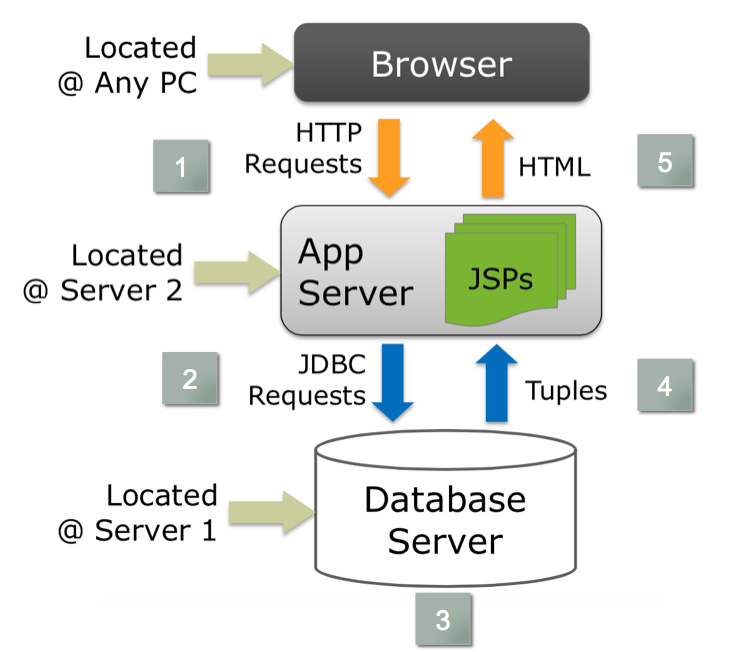
\includegraphics[width=8cm]{images/WebApplicationArchitecture.png}
\caption{Web Application Architecture for Java}
\label{fig:webapp}
\end{minipage} \hfill
\begin{minipage}{0.45\textwidth}
\centering
\begin{Java}[basicstyle=\small]
public List getSumTotals(List selectedNations) {
     List sumTotals = new ArrayList();
     PreparedStatement stmt = conn.prepareStatement(
        "SELECT sum(o.total_price) as sumTotal "
        + "FROM Orders o, Customers c "
        + "WHERE o.cust_ref = c.cust_key "
        + "AND c.nation_ref = ?");
     for (Nation nation : selectedNations) {
         stmt.setInt(1, nation.getNationKey());
         ResultSet rs = stmt.executeQuery();
         rs.next();
         int sum = rs.getInt("sumTotal");
         sumTotals.add(Pair.of(nation, sum));
     }
     return sumTotals;
}
\end{Java}
\caption{Java Code for Example 1}
\label{fig:code1}
\end{minipage} \hfill
\end{figure}


\begin{figure*}[t]
\centering
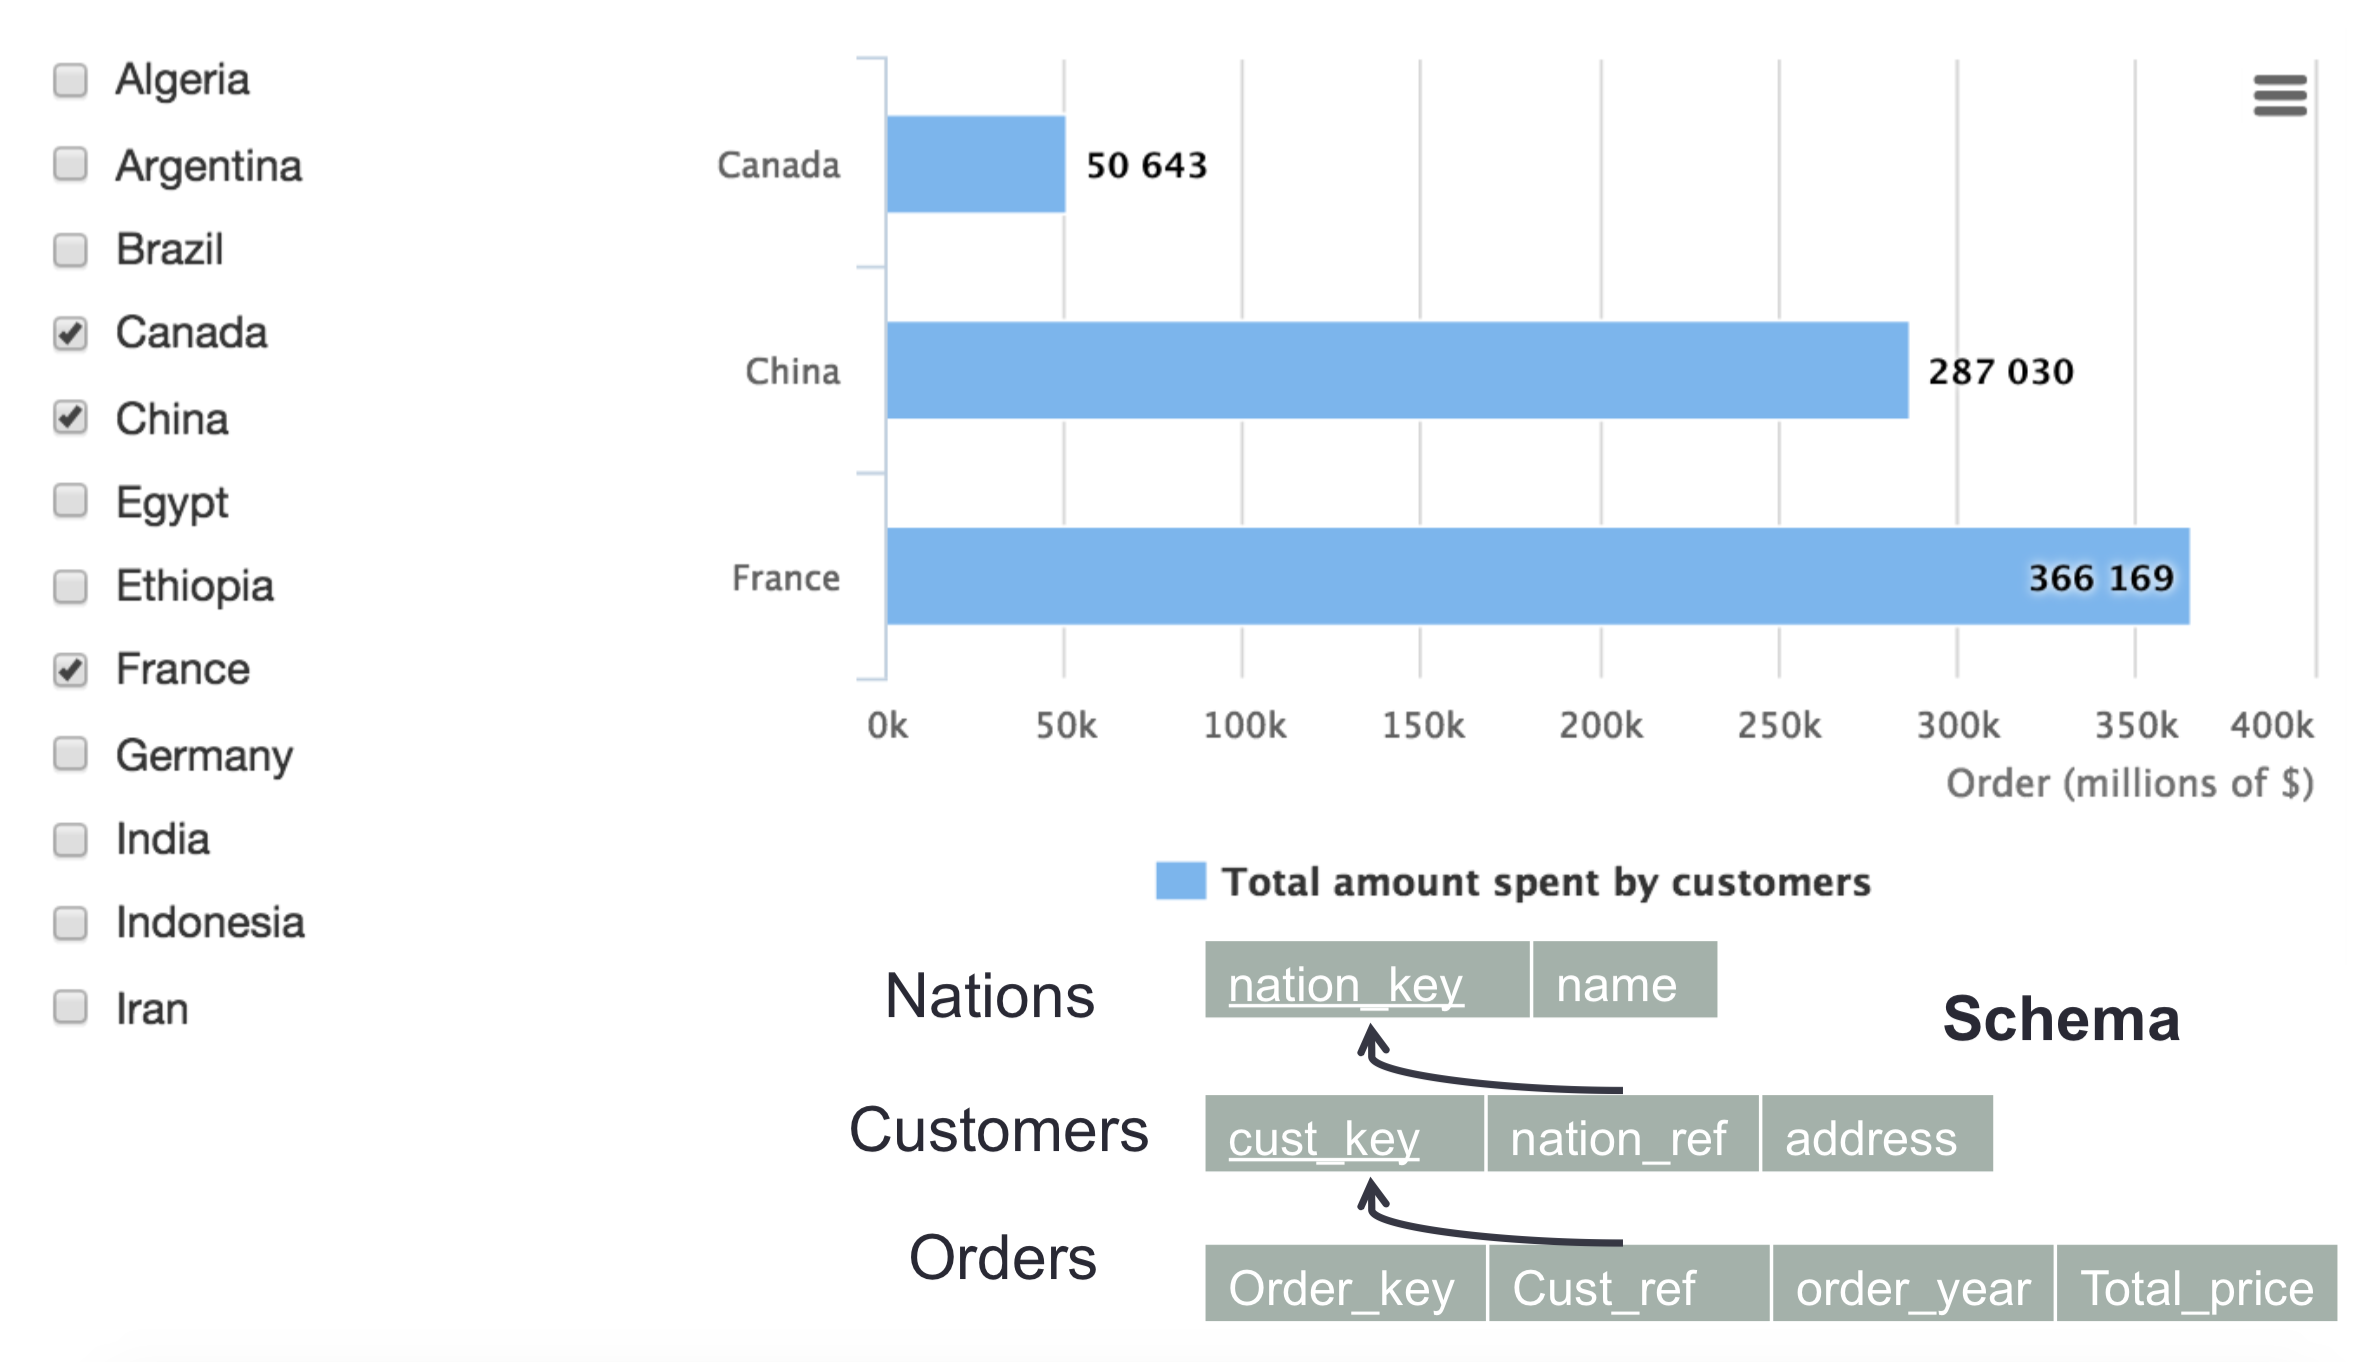
\includegraphics[width=14cm]{images/RunningExample.png}
\caption{Monitor amount spent by customers from selected countries (Example 1)}
\label{fig:example1}
\end{figure*}

To ensure latencies as low as possible, it is important to understand how latency arises. Figure \ref{fig:webapp} describes the architecture of typical web applications and the journey of a user request: \footnote{Note that the architecture on this figure is Java-specific, but the same architecture is used for web application frameworks in other languages such as Python, Ruby or Javascript.} \
\begin{enumerate}
\item{An HTTP request is sent from the browser to the application server, containing the data the user specified when clicking on the web page.}
\item{The request is processed by the application server logic, which in turn sends database queries.}
\item{Each query is compiled, optimized and executed individually.}
\item{The result of the queries are returned to the application program which produces an HTML template with the updated information.}
\item{The HTML result is sent back to the user's browser.}
\end{enumerate}
During this process, latency is dominated by 1) communication over the network in steps 1,2,4,5 (although bandwidth for processing between the application and database servers will typically be higher) and 2) disk I/O to access data from the database.

As a running example, consider the web application shown on Figure \ref{fig:example1}, which describes a dashboard for visualizing and analyzing sales data, based on a TPC-H database \cite{tpch}. A user checks boxes according to the nation she wants to analyze, and the selections are kept as in-memory objects within the HTTP session of the application server. The application then displays an HTML table with the total sales revenue for the selected nations. When the request for new set of checkboxes is issued to the application server, the program on figure \ref{fig:code1} is executed. On line 10, for each \texttt{nation} in the \texttt{selectedNations} list, a parameterized query is issued which computes the desired sum. Each sum computation requires producing a join between two large relations, albeit with a selection on customers based on the nation reference. The results are then accumulated on line 13 and returned for further processing on line 15. We denote this kind of data access pattern a \textbf{parameter-at-a-time} execution.

This execution pattern will iteratively send a SQL query for each requested nation, and each such query will return a single value. This kind of execution comes with two kinds of performance problems : 
\begin{enumerate}
\item{\emph{Network round trip delay}: every SQL query requires a round-trip delay, regardless of the size of the data sent or received. Given that the bandwidth available between an application server and a database server is typically high, and will likely be underused.}
\item{\emph{Repeated disk I/O}:  every SQL query will perform random I/O on the \texttt{Customers} relation followed by a join with the \texttt{Orders} relation, two rather expensive computations.}
\item{\emph{Sequential Execution}: SQL queries are sent to the database sequentially by the application program, which means the latency cost for a single page request will be at least the sum of the costs of each network round trip and disk I/O performed! These queries could, however, be run in parallel.}
\end{enumerate}

Clearly, the parameter-at-a-time execution pattern will be too inefficient if either the data volume or the query load becomes too high. This problem cannot be solved by database compiler alone, because it considers and optimizes each query individually. This problem cannot be solved by the application program compiler either, because the queries are expressed in a language it does not understand (SQL). This problem has been known for decades in the database research community as the impedance mismatch problem \cite{cook:2005aa, maier:1987aa}. The solutions found by researchers over the last decade attempt to solve this problem by \emph{holistic optimization}: making the application compiler aware of database access, giving the query compiler access to more efficient data processing strategies. Notice that while this problem clearly occurs in web applications, it can also occur in non-web applications which make use of a database.

\textbf{Roadmap} Section 2 presents a more efficient data processing strategy, denoted \emph{set-at-a-time} execution, studied by database researchers since the 1980's. Section 3 presents two different approaches to holistic optimization in the research arena which attempt to apply \emph{set-at-time} execution in a database application setting : Query Batching, Query Synthesis. Section 4 presents FORWARD, an all-declarative web application framework developed here at UCSD, which offer a completely different approach in which the application program is also described declaratively; we also compare FORWARD and the other approaches on a number of criteria. Finally in section 5, we propose a future work direction which combines FORWARD and query synthesis to unlock optimization opportunities unavailable before.

\section{Query Decorrelation}

Efficient execution of parameter-at-a-time queries has been a subject extensively studied in the area of database systems in the past  \cite{selinger:1979aa} \cite{dayal:1987aa} \cite{kim:1982aa} \cite{ganski:1987aa} \cite{seshadri:1996aa}. The first paper to show execution of parameter-at-a-time queries was by Selinger  \cite{selinger:1979aa}. In this setting, only the database is considered, there is no application program holding application-resident data, thus in this context \texttt{SelectedNations} is a database relation. Our running example can be then expressed as shown in figure \ref{fig:taat}. This query is then parsed and compiled into a logical query execution plan, which describes how the query can be executed. 

\begin{figure}[h]
\centering
\begin{minipage}{0.45\textwidth}
\centering
\begin{SQL}
SELECT sn.name, (
   SELECT sum(o.total_price) as sumTotal
    FROM Orders o, Customers c
    WHERE o.cust_ref = c.cust_key
    AND c.nation_ref = sn.nation_key
  ) as sumTotal
 FROM SelectedNations sn
\end{SQL}
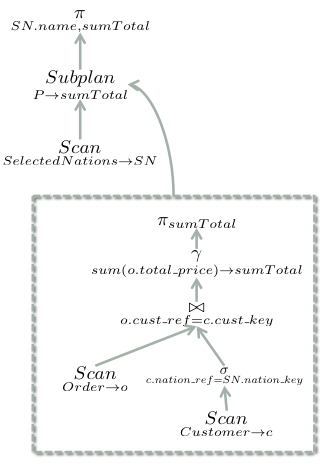
\includegraphics[width=6cm]{images/TAATExecution}
\caption{Parameter-at-a-time Query and Execution}
\label{fig:taat}
\end{minipage} \hfill
\begin{minipage}{0.45\textwidth}
\centering
\begin{SQL}
SELECT SN.name, sum(O.total_price) as sumTotal
FROM SelectedNations SN
LEFT JOIN (Customers C
   JOIN Orders O 
   ON O.cust_ref = C.cust_key)
ON C.nation_ref = SN.nation_key
GROUP BY SN.nation_key, SN.name;
\end{SQL}
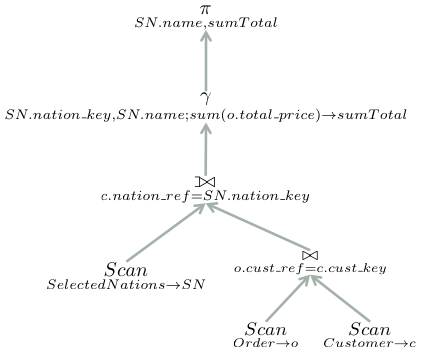
\includegraphics[width=7cm]{images/SAATExecution}
\caption{Set-at-a-time Query and Execution Plan}
\label{fig:saat}
\end{minipage}
\end{figure}

In this execution plan, the subplan operator executes the target query for every selected nation tuple. In each subplan execution, the value \texttt{SN.nation\_key} is parameterized with the value \texttt{nation\_key} column for the \texttt{SN} tuple currently in context. In Selinger's work, this execution plan is followed literally: only the operators within the subplan's inner block are optimized.

Kim \cite{kim:1982aa} was the first to notice that a better evaluation plan was available for such queries, by evaluating all subplans at once, then joining back the result with the outer query. His technique, however, has a bug was discovered by Kiessling \cite{kiessling:1984aa}. The bug was fixed with Dayal's method which introduced the left outer join operator. Dayal's rewriting is shown on figure \ref{fig:saat}. If a selected nation did not have any corresponding customers, Kim's algorithm will not be equivalent to the original plan, while Dayal's algorithm (and all it's successors) do.

Note that Dayal's method can be further optimized by joining a copy of distinct \texttt{SelectedNations} with \texttt{Customers} before the join with \texttt{Orders}. This is the approach taken by Seshadri \cite{seshadri:1996aa}, dubbed \emph{Magic Decorrelation}, which provides a more efficient kind of execution. Even if the number of selected nations is very small, Magic decorrelation (plan on figure \ref{fig:magic}) ensures that only those customers from qualifying nations are fetched, and no more than once.

\begin{figure*}[h]
\begin{minipage}{0.45\textwidth}
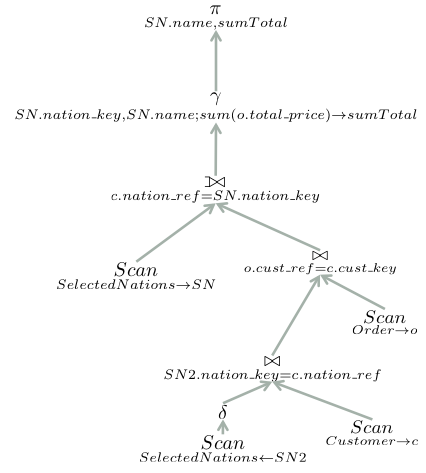
\includegraphics[width=7cm]{images/MagicDecorrelation}
\caption{Magic Decorrelation Execution Plan}
\label{fig:magic}\hfill
\end{minipage}
\begin{minipage}{0.45\textwidth}
\centering
\begin{Java}[basicstyle=\small]
public List getSumTotals(List selectedNations) {
List sumTotals = new ArrayList();
PreparedStatement stmt = conn.prepareStatement( "SELECT sum(o.total_price) as sumTotal "
       + "FROM Orders o, Customers c "
       + "WHERE o.cust_ref = c.cust_key "
       + "AND c.nation_ref = ?");
LoopContextTable lct = new LCT();
int key = nation.getKey();
for (Nation nation : selectedNations) {
    LoopContext ctx= lct.createContext();
    stmt.setInt(1, key);
    ctx.setInt("nation", key);
    stmt.addBatch(ctx);
}
stmt.executeBatch();
for (LoopContext ctx : lct) {
    ResultSet rs = stmt.getResultSet(ctx);
    rs.next();
    int sum = rs.getInt("sum");
    sumTotals.add(Pair.of(nation, sum));
}
return sumTotals;
}
\end{Java}
\caption{Loop Fission}
\label{fig:loopfission}
\end{minipage}
\end{figure*}

Execution plans on figures \ref{fig:saat} and \ref{fig:taat} are semantically equivalent, and the database optimizer can choose either execution to answer the running example query. Which execution plan is the most efficient relies on a number of factors: when the selected nations is very small (just a single nation is selected), the parameter-at-a-time method is actually slightly faster, because fewer operators are used and the subplan is only executed once. As soon as the number of selected nations increases, the magic decorrelation outperforms the parameter at a time execution significantly. That being said, some parameter-at-a-time executions (for example queries with set operators) cannot be rewritten \cite{pirahesh:1992aa} using query decorrelation. However, other techniques are possible, such as caching portions of the subplan which aren't accessed using outer references \cite{rao:1998aa}, since the data they represent do not change between subplan iterations.

Back in the context of web applications, set-at-time execution has the added benefit in web applications to minimize network round-trip delays (only one round-trip is required, no matter how many nations are selected) and  maximizing bandwidth throughput (all the data comes back at once). It can also be applied directly by the programmer, as one can see on figure \ref{fig:code2} (see appendix). In this code fragment, the magic decorrelation evaluation plan is transcribed by the programmer directly in SQL on lines 6-15, while the selected nation keys are added to the SQL query as strings (line 4).

Unfortunately, manually writing a set-at-a-time execution program is cumbersome and error prone. The techniques that we discuss in the next section attempt to solve this problem by allowing programmers to write programs using parameter-at-a-time formulation but have them execute like a set-at-a-time formulation.








\section{Approaches to Holistic Optimization}

\subsection{Query Batching}

Rewriting procedures for batched bindings (or query batching) is a technique developed for the DBridge project  \cite{karthik-ramachandra:2015aa,mahendra-chavan:2011aa,karthik-ramachandra:2011aa,ravindra-guravannavar:2008aa} at IIT Bombay, which attempts to improve database application performance by automatically converting application code fragments exhibiting a parameter-at-a-time execution pattern into fragments exhibiting the set-at-a-time execution pattern.

Guravannavar \cite{ravindra-guravannavar:2008aa} made the following key observation: given that database application programs displaying a parameter-at-a-time execution pattern can be rewritten into a set-at-a-time execution manually, automating this process through program transformation would improve performance of parameter-at-a-time execution code. While Guravannavar focused on database stored procedures, Ramachandra \cite{karthik-ramachandra:2011aa} extended this techniques to Java programs using JDBC \cite{jdbc}.

What he proposes is a source-to-source transformation to rewrite parameter-at-a-time fragments into set-at-a-time fragments, in order to guarantee a more efficient execution. There are, however, limitations to such rewritings, in particular in the presence of side-effects. Guravannavar defines the fragments is able to transform as \emph{batch-safe}. A fragment is said to be batch-safe if the fragment's return value and the system state, for any parameter, are independent from the order in which the parameters are processed.

The transformation process then happens in two steps :
\begin{enumerate}
\item{\emph{Analyze the code fragment} : If the sequence of statements $ss$ in the loop is such that 1) it can be split into two consecutive sub-sequences $ss1$ and $ss2$ such that $ss = ss1 + ss2$ and 2) there are no loop-carried flow/output dependencies \footnote{A loop carried flow (or output) dependency $s_a \rightarrow s_b$ exists if $s_a$ writes a location on iteration $i$, while $s_b$ reads (or writes) from that location on iteration $j$ (where $i < j$).} from any statement in $ss2$ to any statement in $ss$ or the loop predicate, then $ss1$ and $ss2$ can be split into two separate loops. In our example, $ss1$ and $ss2$ correspond to lines 9-10 and 11-13 of figure \ref{fig:code1}, respectively. Loop-carried flow dependencies can be derived from an application program using a \emph{data dependence graph}. The Soot analysis framework \cite{soot} available for Java can produce such a graph.}
\item{\emph{Transform the code fragment}: once the fragment has been identified and validated, it is transformed into the program on figure \ref{fig:loopfission}, in which $ss1$ and $ss2$ are split into two loops.  The responsibility of the first loop is to collect parameters and add them to a \emph{batch table}, whose contents correspond to those of the \texttt{SelectedNations} table from Section 2 when the loop terminates. On line 14, the \texttt{executeBatch()} statement performs the set-oriented execution, by shipping the batch table to the database. On lines 15-20, the second loop's role is to collect the values from the set at a time computations and add them to the sumTotals list in the same order as the original fragment. Finally the \texttt{LoopContextTable} allows the iteration order from the first loop to be preserved in the second loop.}
\end{enumerate}

While this technique converts efficiently fragments which exhibit the parameter-at-a-time pattern, it is limited to code fragments situation where the data-source can supported set-oriented execution, which is not the case, for example, of many web services.
Moreover, the rewriting can only be applied when the initial code fragment is batch-safe, and a small modification (such as side-effecting operation modifying the system state) can violate the conditions for transformations and disable the optimization opportunity. An alternative researchers have explored consists to send multiple queries asynchronously and later retrieved the results \cite{ramachandra:2012aa, manjhi:2009aa}. 




\subsection{Query Synthesis}

Query synthesis is a recent approach at MIT by Cheung  et al., implemented through the QBS algorithm \cite{alvin-cheung:2013aa,alvin-cheung:2013ab}. Instead of trying to target the parameter-at-a-time problem specifically, Cheung uses his technique to obtain the declarative intent of imperative programs which are equivalent to some relational operation. This approach had been previously explored in the context of selections and projections \cite{wiedermann:2008aa}, but Cheung provides the first solution which is applicable to joins and aggregations as well. This kind of optimization is particularly important for programs written using ORMs (Object-Relational Mapping), such as Hibernate \cite{hibernate} for Java, Rails for Ruby \cite{rails} and Django for Python \cite{django}. ORM layers tend to incite programmers to write code that iterates over collections of database records, performing imperatively operations such as join or filters. 

\begin{figure*}[h]
\begin{minipage}{0.45\textwidth}
\centering
\begin{Java}[basicstyle=\small]
long getSumTotalForAlgeria() {
  List customers = customerDao.getAllCustomers();
  List orders = orderDao.getAllOrders();
  long sum = 0;
  for (Customer c : customers)
    for (Order o : orders)
      if (c.getCustKey() == o.getCustRef()
          && c.getNationRef() == 1)
        sum += o.getTotalPrice();
  return sum;
}
\end{Java}
\caption{Find total amount spent by customers from Algeria}
\label{fig:algeria-initial}
\end{minipage}\hfill
\begin{minipage}{0.45\textwidth}
\centering
\begin{Java}[basicstyle=\small]
getSumTotalForAlgeria() {
   List customers = query("SELECT * FROM Customers");
   List orders = query("SELECT * FROM Orders");
   int result = 0; int i,j = 0;
  while (i < size(customers)) { j=0;
    while (j < size(orders)) {
      if (customers[i].cust_key == orders[j].cust_ref && customers[i].nation_ref == 1)
         result += o.total_price;
     j++;
     }
   i++;
   }
   return result;
}
\end{Java}
\caption{Fragment converted to kernel code}
\label{fig:algeria-kernel}
\end{minipage}\hfill
\end{figure*}

\begin{figure*}[h]
\begin{minipage}{0.45\textwidth}
\centering
\textbf{Translated Code} :
\begin{Java}[basicstyle=\small]
  getSumTotalForAlgeria() {
  return db.executeQuery(
    "SELECT sum(total_price) as sumTotal " +
    "FROM Orders o, Customers c " +
    "WHERE o.cust_ref = c.cust_key " +
    "AND c.nation_ref = 1 " +
    "ORDER BY c.cust_key, o.cust_ref"
  );
}
\end{Java}
\caption{Post-Condition and code fragment converted to SQL}
\label{fig:algeria-optimized}
\end{minipage} \hfill
\begin{minipage}{0.45\textwidth} 
\centering
\textbf{Post-Condition}:
\begin{align}
\begin{split}
\centering
& result = sum(\underset{l}{\pi}(\underset{\phi_0 \wedge \phi(1)}{\bowtie}(customers, orders) \\
& \text{where} \\
& \phi_0(e) : e_{nation\_ref} = 1 \\
& \phi_1(e_c, e_o) : e_c.cust\_key = e_o.cust\_ref \\
& l : total\_price
\end{split}
 \label{eq:postcondition}
\end{align}
\end{minipage} \hfill
\end{figure*}

The code on figure \ref{fig:algeria-initial} correspond to a java code fragment semantically equivalent to the query from example 1, expressed specifically for Algeria (the $nation\_key$ attribute for the Algeria nation is 1). This fragment makes use of the Hibernate \cite{hibernate} ORM. On lines 2-3 of figure \ref{fig:algeria-initial}, the entire customers and orders relations are requested from the database as Java lists. Unfortunately, the ORM library is unaware of the relational operations on lines 5-8, therefore cannot utilize indices or efficient join strategies from the database and has to fetch the contents of the entire order and customer relations. On line 10, the computed sum is returned. 

The goal of query synthesis is to identify code fragments like the one on figure \ref{fig:algeria-initial} and transform them into the fragment shown on figure \ref{fig:algeria-optimized}. Cheung relies on the observation made by Iu et al. \cite{iu:2010aa} that if one can express a post-condition from imperative code in relational algebra, then that block can be translated into SQL. The goal is thus to derive loop invariants and a post-condition for the value of the variable returned at the end of the fragment (this variable is dubbed the \emph{result} variable). In our running example context, the result variable would be \texttt{sum}. 

To express post-conditions and invariants, Cheung designed a theory which he called the Theory of Ordered Relations (TOR). This theory can be understood as relational algebra defined over lists instead of sets. Being able to reason about the order of records matters for two reasons : 
\begin{enumerate}
\item{The invariants may have to express partially constructed lists. In our running example, they must express the fact that the sum is computed from the first $i$ and $j$ records from $customers$ and $orders$, respectively.}
\item{Nested loops may impose an order on the result list which might be used by the application, even when the original lists are ordered arbitrarily.}
\end{enumerate}

\begin{table}[h]
\centering
\begin{tabular}{|p{5cm}|p{10cm}|}
\hline
Inner loop preservation & $j < size(orders) \wedge \textbf{iInv}(i,j,customers, orders, result) \rightarrow (\theta(customers, orders) \wedge \textbf{iInv}(i,j+1, customers, orders, result +
get_j(orders).total\_price)) \vee (!\theta(customers, orders) \wedge \textbf{iInv}(i,j+1, customers, orders, result))$ \\ \hline
Outer Loop Exit & $i \geqslant size(customers) \vee \textbf{oInv}(i, customers, orders, result) \rightarrow \textbf{pCon}(result, customers, orders)$ \\ \hline
\multicolumn{2}{|p{14cm}|}{where $\theta(customers, orders):= get_i(customers).cust\_key = get_j(orders).cust\_ref \wedge get_i(customers).nation\_ref = 1$} \\
\hline
\end{tabular}
\caption{Two of the verification conditions for the running example}
\label{table:vc}
\end{table}

\begin{figure*}[h]
\centering
\begin{align*}
& \textbf{oInv}(i,customers,orders,result) : \\
& i \leqslant size(customers) \wedge result = sum(\underset{l}{\pi}(\underset{\phi_0 \wedge \phi_1}{\bowtie}(top_i(customers), orders))) \\
& \textbf{iInv}(i,j,customers,orders,result) : \\
& i < size(customers) \wedge j \leqslant size(orders) \wedge result = sum( \\
& \text{  } \underset{l}{\pi}(\underset{\phi_0 \wedge \phi_1}{\bowtie}(top_i(customers), orders))) \\
& \text{  } + \underset{l}{\pi} (\underset{\phi_0 \wedge \phi1}{\bowtie}(get_i(customers), top_j(orders))) \\
& \textbf{pCon}(customers,orders,result) : \\
& result = sum(\underset{\phi_2}{\pi}(\underset{\phi_1 \wedge \phi_0}{\bowtie}(customers, orders))) \\
& \text{where} \\
& \phi_0(e) : e_{nation\_ref} = 1 \\
& \phi_1(e_c, e_o) : e_c.cust\_key = e_o.cust\_ref \\
& l : total\_price
\end{align*}
\caption{Invariants and post-condition found}
\label{eq:found}
\end{figure*}


The transformation process happens in 5 steps :
\begin{enumerate}
\item{\emph{Identifying code fragments and conversion to kernel code}: note that this algorithm is applied on large-scale software projects, with multiple thousands of lines of code. To this effect, the algorithm starts by searching the software code for potential code transformation targets. Real-world programs introduce the complexity of aliasing and method calls, which may hide opportunities for conversion. For example, the code transformation in our running example would not be possible without knowing that the \texttt{getAllCustomers} and \texttt{getAllOrders} methods execute queries on the database and returned non-aliased lists of results. Once a target is found, it transforms the expression into simplified kernel language. The kernel language version is available on figure \ref{fig:algeria-kernel}. In the kernel language, aliases and method calls are inlined, and Hibernate data persistence methods are replaced with the \texttt{Query(...)} construct (lines 2-3 of figure \ref{fig:algeria-kernel}).}
\item{\emph{Computing Verification Conditions}: as a next step, the verification conditions of the code fragment expressed in the kernel language are computed. These verification conditions are expressed using TOR and computed using standard techniques from axiomatic semantics. Two of the verification conditions generated by the algorithm are shown on table \ref{table:vc}. The inner and outer loops refer here to the loops on lines 5 and 6 of figure \ref{fig:algeria-kernel}, respectively. The first assertion presents an inductive argument that the inner loop invariant is preserved after one iteration of the nested loop. The $result$ variable is incremented by $get_j(orders).total\_price$ if the condition $\theta(customers, orders)$ is met, and remains unchanged otherwise. The second assertion ensures the post-condition will be true when the outer-loop terminates. } 
\item{\emph{Produce and validate loop invariants and post-condition candidates}: notice that this verification conditions treat the loop invariants and post-condition as unknown predicates ("holes") over the variables currently in scope when the loop is entered. The goal of this algorithm is to fill the holes in a way which validates the verification conditions. This is done through constraint-based synthesis \cite{solar-lezama:2006aa}, which will search the space of possible completion of the holes for one that is valid according to a bounded model-checking procedure. The Z3 \cite{Z3} theorem prover is used for the validation. The valid candidates found for our running example are shown on figure \ref{eq:found}. The output invariant (\textbf{oInv}) ensures that at the $i$th iteration of the outer loop, the $result$ variable has a value equal to the sum of the order total prices for the first $i$ customers. The input invariant (\textbf{iInv}) ensures the top $j$ orders for the $i$th customer are added to the result variable. Finally the post-condition ensures the result variable is equal to the sum of all the order prices.}
\item{\emph{Convert the post-condition into SQL}: the post-condition found can finally be translated to SQL using a set of  syntactic rules. Note the introduction of the \texttt{ORDER BY} clause on figure \ref{fig:algeria-optimized}. This clause is added in order to satisfy the ordering semantics of TOR expressions, although is completely useless in this situation, since only the sum is required. It is up to the query compiler to realize that the data does not need to be ordered in this situation, and remove the expensive sorting.}
\end{enumerate}

This approach has the advantage to be much more versatile than the query batching technique, allowing to transform a wide variety of code fragments, from joins to filters to aggregations. It is, however, not adapted to the parameter-at-a-time problem exactly, because the kernel language does not currently provide a way to represent parameterized queries nor does it provide a way to ship application data to the database.

\section{FORWARD}

\subsection{Declarative Web Application Frameworks}

\begin{figure*}[h]
\centering
\begin{minipage}{0.45 \textwidth}
\centering
\begin{SQL}[basicstyle=\small, language=HTML]
<fstmt:with target="shown_nations">
SELECT sn.name, (
    SELECT sum(o.total_price) as sumTotal
    FROM db.Orders o, db.Customers c
    WHERE o.cust_ref = c.cust_key
    AND c.nation_ref = sn.nation_key
) as sumTotal
FROM session.SelectedNations sn
</fstmt:with>
<funit:bar_chart>
  <fstmt:for source="shown_nations">
    <column>
      <label> {sn.name} </label>
      <value> {sumTotal} </value>
    </column>
  </fstmt:for>
</funit:bar_chart>
\end{SQL}
\caption{FORWARD Page}
\label{fig:forward-code}
\end{minipage} \hfill
\begin{minipage}{0.45\textwidth}
\centering
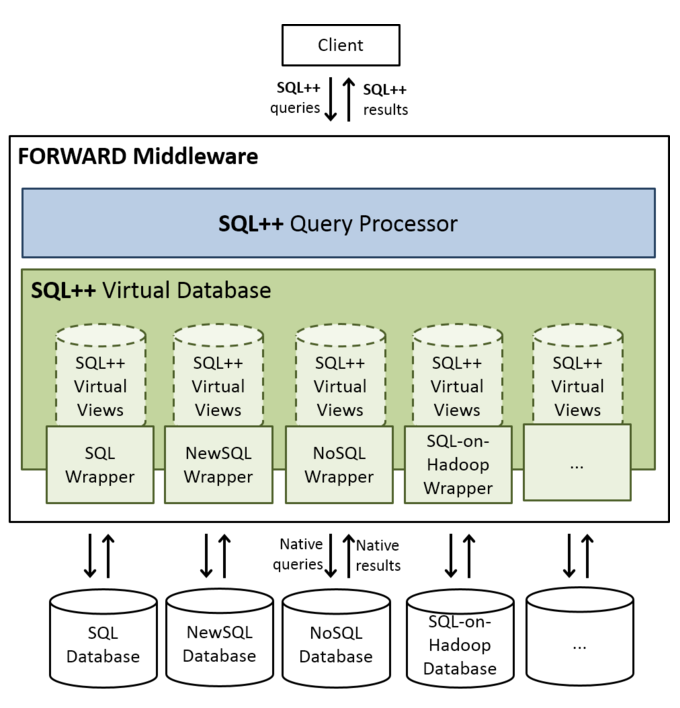
\includegraphics[width=8cm]{images/architecture}
\caption{FORWARD Architecture}
\label{forward}
\end{minipage}\hfill
\end{figure*}

The previous works we have have all tried to improve the performance of the application program expressed using an imperative language. FORWARD \cite{kian-win-ong:2014aa, yupeng-fu:2014aa} presents a completely different approach in which the entire application is expressed declaratively using a single language: SQL++. SQL++ is backwards compatible with SQL while supporting the JSON \cite{JSON} data model, the data model behind many NoSQL applications which also integrates easily with application programming objects. The FORWARD web application framework (see figure \ref{forward}) provides a query processor located on the application server, which can derive multiple execution plans for a given SQL++ query, and pick the one with the smallest cost, the same way a cost-based database query optimizer would, but in a distributed environment.

FORWARD allows the developer to write the running example using a page query (see figure \ref{fig:forward-code}), in which both the data access code and the visualization code are represented. The SQL++ query language is \emph{distributed}, with data being accessed both from the application and the database(s) being seamlessly integrated.  For example, on figure\ref{fig:forward-code}, data is being accessed on line 3 from the database, and on line 8 from the HTTP browser session of the user currently browsing the page. The semantics of the \texttt{fstmt:for} statement (lines 11-16) are to evaluate the query in the \texttt{fstmt:with} clause and output its body for every record in the query's response.

The FORWARD engine is a middleware installed on the application server which includes a query processor which evaluates queries based on a number of virtual views, each view corresponding to data located either on locally (on the application server, for example the HTTP session), or externally in a database. The FORWARD query processor operates in 5 stages :

\begin{figure*}[h]
\centering
\begin{minipage}{0.45\textwidth}
\centering
\begin{SQL}[basicstyle=\small, language=HTML]
SELECT SN.name, sum(O.total_price)
FROM (
  SELECT *
  FROM Nations N
  WHERE N.nation_key IN (4,5,8)
) SN
LEFT OUTER JOIN Customers C
JOIN Orders O 
ON O.cust_ref = C.cust_key
ON C.nation_ref = SN.nation_key
GROUP BY SN.name;
\end{SQL}
\caption{Query sent by FORWARD middleware to database}
\label{fig:forward-query}
\end{minipage} \hfill
\begin{minipage}{0.45\textwidth}
\centering
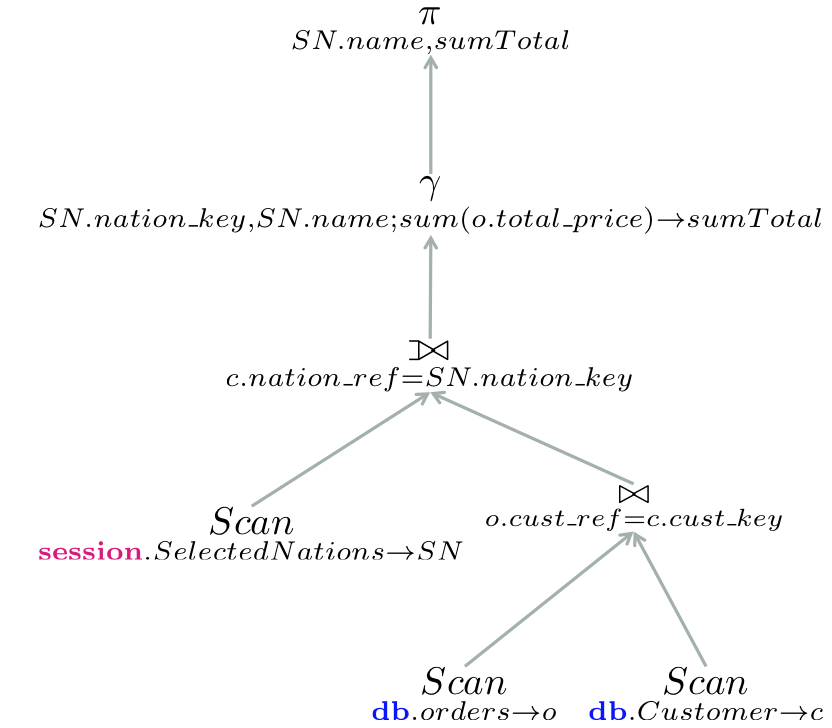
\includegraphics[width=8cm]{images/distributed-plan}
\caption{Distributed Execution Plan}
\label{fig:distributed}
\end{minipage} \hfill
\end{figure*}

\begin{enumerate}
\item{\emph{Syntax Analysis}: the SQL++ queries are parsed into an abstract syntax tree (AST).}
\item{\emph{Initial plan translation \& Source Agnostic Rewritings}: the AST is then converted into a logical plan which is then optimized using source-agnostic rewriting rules. The set-at-a-time execution plan rewriting is a source agnostic rewriting which would be executed at this step. In our running example, the execution plan at this step would be correspond to the set-at-a-time execution plan shown on figure \ref{fig:distributed}. Notice that this plan is distributed, with \texttt{session} and \texttt{db} annotations indicating that the relation is application-resident and database-resident, respectively.}
\item{\emph{Plan Distribution \& Source Specific Rewritings}: The query processor decides where each operation will be computed. In our running example, the query processor will realize that the most efficient execution should ship the data from the \texttt{selectedNations} relation to the \texttt{db} database, and execute the set-at-time join there.}
\item{\emph{Physical Plan Generation \& Native Query Generation}: The distributed query plan is converted into the SQL query shown on figure \ref{fig:forward-query}. Notice that the query exhibits the set-at-a-time execution pattern and sends over the values (4,5,8), which corresponds to the \texttt{nation\_key} attributes of the nations currently selected by the user. }
\item{\emph{Plan Execution}: The generated query is sent to the \texttt{db} database, the results are retrieved by FORWARD and then used to populate the page.}
\end{enumerate}

Note that the distributed query execution and optimization is only one of FORWARD's characteristics. FORWARD also uses incremental view maintenance \cite{fu:2011aa}, to ensure that whenever a collection is updated either on the browser session or on one of the database instances, the change is reflected on the user's browser. 

\subsection{Beyond SQL}

\begin{figure*}[!ht]
\centering
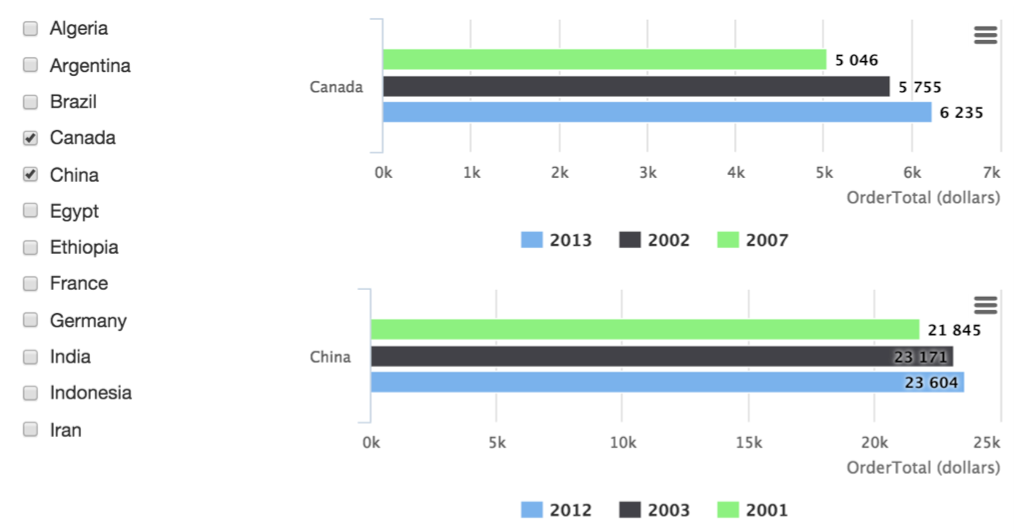
\includegraphics[width=14cm]{images/complex-example}
\caption{Monitor Top 3 Years of amount spent for selected countries (Example 2)}
\label{fig:complex-example}
\end{figure*}

\begin{figure*}[p]
\centering
\begin{minipage}{0.45\textwidth}
\centering
\begin{Java}[basicstyle=\small]
public List getSumTotal3Years(List selectedNations)  {
  List sumTotals = new ArrayList();
  PreparedStatement stmt = conn.prepareStatement(
      "SELECT order_year, sum(o.total_price) as sumTotal\n"
   + "FROM Orders o, Customers c\n"
   + "WHERE o.cust_ref = c.cust_key\n"
   + "AND c.nation_ref = ?\n"
   + "GROUP BY o.order_year\n"
   + "ORDER BY sumTotal DESC\n"
   + "LIMIT 3");
   for (Nation nation : selectedNations) {
      stmt.setInt(1, nation.getNationKey());
      ResultSet rs = stmt.executeQuery();
      List pairs = new ArrayList();
      while (rs.next()) {
         int year = rs.getInt("order_year");
         int total = rs.getInt("sumTotal");
         pairs.add(Pair.of(year,total));
      }
      sumTotals.add(pairs);
   }
   return sumTotals;
}
\end{Java}
\caption{Java Code for Example 2}
\label{fig:code-complex}
\end{minipage} \hfill
\begin{minipage}{0.45\textwidth}
\centering
\begin{SQL}
SELECT n.nation_key, n.name, (
  SELECT order_year,
         sum(total_price) as sum_price
  FROM db.orders AS o,
       db.customers AS c
  WHERE o.cust_ref = c.cust_key
  AND c.nation_ref = n.nation_key
  GROUP BY order_year
  ORDER BY sum_price DESC
  LIMIT 3
) AS aggregates
FROM session.selected_nations AS s,
     db.nations AS n
WHERE s.nation_ref = n.nation_key
AND  s.selected = true
\end{SQL}
\caption{SQL++ Code For Example 2}
\label{fig:complex-query}
\end{minipage} \hfill
\centering
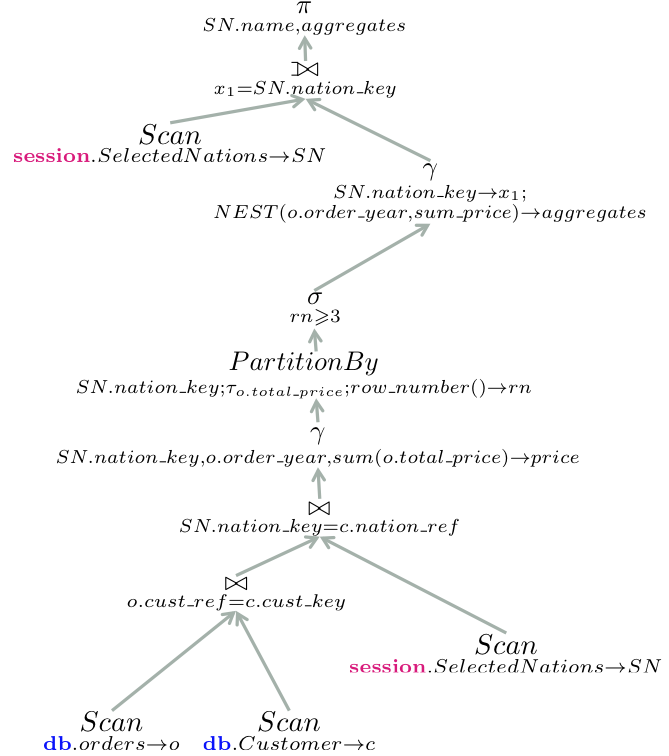
\includegraphics[width=8cm]{images/distributed-complex-plan}
\caption{Set-at-a-time rewritten plan for example 2}
\label{fig:complex-example-plan}
\end{figure*}

Consider the extension to the running example shown on figure \ref{fig:complex-example}, in which the top three years of sales revenue are displayed instead of the total revenue across all years. The Java code for this extension using the parameter-at-a-time technique is shown on figure \ref{fig:code-complex}.

The query shown (on lines 4-10), computes the top three years in terms of sales revenue for a parameterized nation. The lines 15 to 18 collects the year and sum into a list called \texttt{pairs} before adding them to the output list. In this situation, for each parameterized query, a \emph{list} of values is obtained from the database instead of a scalar. In this situation, the batched form of the complex  would violate the first normal form, and cannot be expressed using SQL. In this context, the query batching and query synthesis approaches, which are based on the relational data model, can't be used. 

SQL++, however, can operate over semi-structured data. Figure \ref{fig:complex-query} shows a SQL++ query for example 2. Lines 2-10 display a \emph{correlated subquery} which returns the 3 top years for the nation bound to variable $n$.

The FORWARD query processor represents a correlated subquery using the \emph{ApplyPlan} operator, which takes as input a semi-structured record $t = \{a_1:v_1, ..., a_n:v_n\}$ and a plan $p$. It evaluates plan $p$ over $t$ to value $w$, and outputs a new record $\{a_1:v_1, ..., a_n:v_n, b:w\}$. Note that values $v_1, ..., v_n, w$ may be themselves scalars, records, or even list of records. Note that variables $a_1,...,a_n$ of the input binding tuples appear as parameters in $p$ wherever constants or variables can appear in uncorrelated plans. The \emph{GroupBy} operator (also denoted $\gamma$) can also generate nesting, through the \emph{Nest()} aggregate function, which instead of outputting a scalar outputs the list of records with the same grouping values. 

In our running example, the FORWARD query processor parses the query on figure \ref{fig:complex-query} and produces an initial logical plan using the ApplyPlan operator. It then removes the apply-plan operator using a set-at-a-time rewriting rule \cite{yupeng-fu:2014aa} and produces the distributed plan shown on figure \ref{fig:complex-example-plan}. This plan has a number of differences with the relational set-at-a-time plan : 

\begin{itemize}
\item{Notice that the nesting in the rewritten plan is produced by a $\gamma$ operator with the \emph{Nest()} aggregation function. Given that the \emph{Nest()} aggregation cannot be performed by the relational database, it is performed by the FORWARD middleware.}
\item{The \emph{PartitionBy} operator applies the ordering over the partitions formed by the nation keys, which allows the sorting of the different groups within the relational database.}
\end{itemize}

Only a single denormalized query is sent from to the database in this example, while the \emph{Nest()} aggregation function is used to create the nested lists. 

\subsection{Integrated Query Languages}
%% Short Version

Another approach taken by researchers to integrate nested data into application programming languages has been through \emph{Integrated Query Languages}. One of the most popular implementations is Microsoft's LINQ \cite{LINQ},  which integrates seamlessly a declarative query facility within the application programming language. With LINQ, developers use Standard Query Operators (SQOs) to formulate queries against both application objects, database-resident data and XML files. The queries are eventually translated into SQL or XQuery if they target database data or XML data, respectively. Here is an example of a LINQ program for Example 2. On line 1, the \texttt{n} variable is bound to the table \texttt{nations} and filtered according to the \texttt{Where} SQO. The \texttt{Select} SQO is used lines 2-10 to collect the top 3 years data. This code will also produce a parameter-at-a-time execution, as LINQ will produce a separate SQL query for each invocation of the \texttt{Select} SQO. 

\begin{SQL}
var result =
	from n in db.nations
	where selectedKeys.Any(key => key == n.nation_key))
	select new {
		name = n.name,
		aggregates = (from c in db.customers
		where c.nation_ref equals n.nation_key
		join o in orders on c.cust_key == o.cust_ref
		group o by o.order_year into g
		select new {
			order_year = g.order_year,
			sum_total = g.sum(t => t.total_price)} into ag
		orderByDescending ag.sumTotal
		limit 3)
	}
\end{SQL}

Gurst \cite{gurst:2010aa} presents a way to translate the SQOs into algebraic plans through a technique called \emph{loop lifting} \cite{gurst:2004aa, gurst:2009aa}. The algebraic plans themselves can then be translated to SQL. A single LINQ query translation can have multiple plan roots, possibly with common-subexpressions. However, the number of plan roots is limited by level of nesting in the query result type. This technique guarantees that it is only a LINQ query's static result type, and not the size of the database, which determines the number of SQL queries produced. Gurst extended his work to the Ruby programming language with the SWITCH tool \cite{gurst:2013aa}. 


\subsection{Comparison with other approaches}

\begin{table*}[h]
\centering
\caption{Comparison of holistic optimization frameworks}
\label{table:comparison}
\begin{tabular}{|c|c|c|c|c|c|c|c|}
\hline
Approach & Framework  & A   & B   & C   & D     & E           & F   \\ \hline
Declarative Middleware & FORWARD & Yes & N/A & Yes & SQL++ & Declarative & Yes \\ \hline
Query Batching  & DBridge & Yes & No  & No  & Java  & Imperative  & No  \\ \hline
Query Synthesis & QBS & No  & Yes & No  & Java  & Imperative  & No  \\ \hline
Integrated Query Language & LINQ & Yes & N/A & Yes & C\#/Visual Basic & Declarative & Yes \\ \hline
\end{tabular}
\caption*{
    \begin{tabular}{l l}
      A: & Enables set-at-a-time execution \\
      B: & Enables database execution of imperative code fragments\\
      C: & Requires special syntax / custom language \\
      D: & Application programming language \\
      E: & Application programming paradigm \\
      F: & Targets Nested Relational Data
    \end{tabular}
}
\end{table*}

A comparison of the different holistic optimization approaches is shown on table \ref{table:comparison}. Both the declarative middleware and query batching approaches allow the optimization of the parameter-at-a-time execution into set-at-a-time execution, but not Query Synthesis. Note, however, that the Query Batching and Query Synthesis procedures can be applied on the same codebase, given they are independent techniques which do not require special syntax, and both approaches have a java implementation : QBS and DBridge.  Query synthesis is the only approach which can recognize and transform imperative fragments into SQL. Both Query Synthesis and Query batching can be applied to fragments written using an imperative style, while FORWARD and LINQ are the only approaches which can optimize a nested relational data access.

\section{Conclusion and Future Work}

This paper describes the challenges posed by the impedance mismatch between application and database compilers in the typical web/database application architecture, and the holistic optimization solutions found in previous works. We show that the query synthesis and the query batching approaches can be applied on different kinds of imperative application programs, while declarative middleware such as FORWARD provide holistic optimization over both structured and semi-structured data, which becomes increasingly important with the advent of NoSQL databases.

However, declarative middlewares are fundamentally limited by the fact that it requires a declarative programming paradigm in order to leverage its power query processing capabilities. Web developers, on the other hand, are used to program using imperative programming languages with ORMs. Our idea for future work would be to use program transformation techniques seen in section 3 to convert application programs written in a imperative style into SQL++ programs which can be run on the FORWARD middleware. According to past database research, a report over a database can be modeled by a single semi-structured query. Thus, if one is able to convert the entire data access made by an application program into a single SQL++ query, then the data access can be holistically optimized. The versatility of the query synthesis technique may proves to be a good candidate for such a venture. There are, however, at least two immediate hurdles to that effort:

\begin{itemize}
\item{\emph{Synthesize parameterized queries}: the current query synthesis algorithm does not synthesize parameterized queries, which would be necessary to take advantage of FORWARD's powerful query decorellation capabilities.}
\item{\emph{Synthesize semi-structured data}: the TOR theory is defined over lists of records, while synthesizing semi-structured would require a theory capable of expressing both nesting and heterogeneity.}
\end{itemize}

Understanding how to overcome these obstacles is being currently investigated. 

\bibliography{bibliography}{}
\bibliographystyle{plain}
\titleformat{\section}{\large\bfseries}{\appendixname~\thesection .}{0.5em}{}

\begin{appendices}
\begin{figure}[h]
\centering
\begin{Java}[basicstyle=\small]
public List getSumTotals(List selectedNations) {
     List sumTotals = new ArrayList();
     // Generates a string "(1,2,3)" if nations with id 1,2 and 3 were selected
     String keysString = makeString(selectedNations);
     PreparedStatement stmt = conn.prepareStatement(
        "WITH (SELECT DISTINCT * "
        + "FROM Nations WHERE nation_key IN " + keysString
        + ") AS Temp"
        +  "SELECT SN.nation, sum(o.total_price) as sumTotal "
        + "FROM Nations SN LEFT OUTER JOIN ("
        + "Temp SN2, Orders o, Customers c "
        + "WHERE o.cust_ref = c.cust_key"
        + "AND SN2.nation_key = c.nation_ref)"
        + "AND c.nation_ref = SN.nation_ref"
        + "AND SN.nation_key IN " + keysString);
     while (rs.next()) {
     	nation = rs.getString("nation");
	sum = rs.getInt("sumTotal");
     	sumTotals.add(Pair.of(nation,sum));
     }
     return sumTotals;
}
\end{Java}
\caption{Java Code for Example 1 using Set-at-a-time execution}
\label{fig:code2}
\end{figure}
\end{appendices}
\end{document}